\documentclass[letterpaper,12pt,fleqn]{article}
\usepackage[margin=64pt]{geometry}
\usepackage{amsthm}
\usepackage{amsmath}
\usepackage{amssymb}
\usepackage{parskip}
\usepackage{graphicx}
\usepackage{enumerate}
\usepackage{xcolor}
\usepackage{hyperref}


\newcommand{\transpose}{^{\mbox{\tiny T}}}


\begin{document}
\pagestyle{empty}

\hrule \vspace{0.5em}
\noindent {\bf CFRM 410} \hfill Assignment 1 \newline \hrule

\vspace{1em}

The first three exercises are calculus and linear algebra review. If you are unable to do these exercises% you should expect to have significant mathematical difficulties later in the course.

\begin{enumerate}
\item Let
\begin{equation*}
f(x) = \frac{1}{2a} \log \left| \frac{x - a}{x + a} \right| + b
\end{equation*}
where $a > 0$ and $b$ are constants, $\log$ denotes the natural logarithm, and $| \cdot |$ denotes the absolute value.

\begin{enumerate}[a)]
\item What is the domain of $f(x)$?

The largest possible domain for $f$ is $D = \mathbb{R} \backslash \{-a,a\}$ since $| \cdot | \geq 0 \; \forall x \in \mathbb{R}$ and the real valued log function $log(y)$ may be defined sensibly only for $y > 0$.

\item Compute $f'(x)$.

First we show for $u : D \subset \mathbb{R} \longrightarrow \mathbb{R}$, that wherever $|u(x)|$ is differentiable, its derivative is given by $\frac{u(x)u'(x)}{|u(x)|}$:

$$ \frac{d}{dx} |u(x)| = \frac{d}{dx} \sqrt{(u(x))^2} = \frac{1}{2\sqrt{(u(x))^2}}2u(x)u'(x) = \frac{u(x)u'(x)}{|u(x)|}.$$

Using this we have
$$f'(x) = \frac{1}{2a}\left|\frac{x+a}{x-a}\right|\frac{\frac{x-a}{x+a}\frac{x+a-(x-a)}{(x+a)^2}}{\left|\frac{x-a}{x+a}\right|} = \frac{1}{2a}\frac{|(x+a)^2|}{|(x-a)^2|}\frac{2a(x-a)}{(x+a)^3} = \frac{1}{x^2-a^2} \; (x \neq \pm a).$$

\item Evaluate the indefinite integral
\begin{equation*}
\int \frac{1}{x^{2} - 2x} \, dx
\end{equation*}
by completing the square.

\begin{align*}
\int \frac{dx}{x^2-2x+1-1} &= \int \frac{dx}{(x-1)^2 - 1} \quad \left(x-1 = sec\theta \implies dx = sec\theta tan\theta d\theta\right) \\
&= \int \frac{sec\theta tan\theta d\theta}{sec^2 \theta - 1} \\
&= \int \frac{sec\theta d\theta}{tan\theta} \\
&= \int csc\theta d\theta \\
&= -log|csc\theta + cot \theta| +c \quad(*) \\
&= -log \left|\frac{x-1}{\sqrt{x^2-2x}} +\frac{1}{\sqrt{x^2-2x}}\right| + c \\
&= log \left|\frac{\sqrt{x(x-2)}}{x} \right| + c \\
&= log|\sqrt{x(x-2)}| - log|x| + c \\
&= \frac{1}{2}(log|x| + log|x-2|) - log|x| + c \\
&= \frac{1}{2}(log|x-2| - log|x|) + c.
\end{align*}
(*) Here we used a standard integral list found at https://en.m.wikipedia.org/wiki/ \;.
\end{enumerate}

\vspace{2em}


\item Let $D$ be the region in the $xy$-plane bounded by the parabolas $y = 2x^{2}$ and $y = 1 + x^{2}$ and satisfying $|x| < 1$.

\begin{enumerate}[a)]
\item Sketch the region $D$.

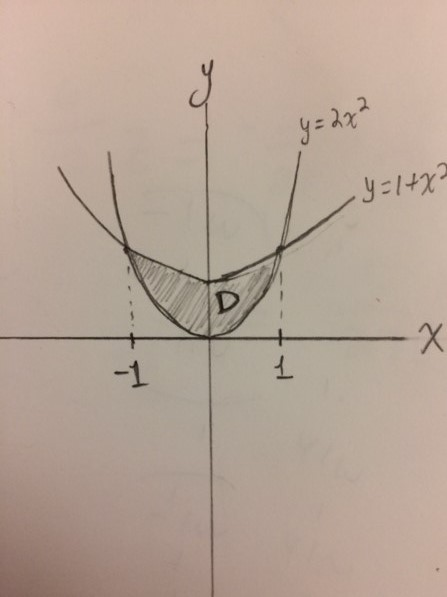
\includegraphics[scale=0.25]{Region}

\item Evaluate the definite integral
\begin{equation*}
\iint_{D} x^{2} \, dA = \int_{-1}^{1} \int_{2x^2}^{1+x^2} x^2 \; dy\,dx = \int_{-1}^{1} x^2y \big\rvert_{2x^2}^{1+x^2} \;dx = \int_{-1}^{1} x^2-x^4 \;dx = \frac{x^3}{3}-\frac{x^5}{5}\big\rvert_{-1}^{1}=\frac{4}{15} \;.
\end{equation*}

\end{enumerate}

\vspace{2em}


\item ** For problems 3 and 4 I have included in this document snippets of R code used for each problem. However, I have also attached all the code collected together in a seperate document submitted as well to possibly assist in grading.**

Let
\begin{equation*}
{\bf A} = \begin{bmatrix} 1 & 4 \\ 2 & 5 \\ 3 & 6 \end{bmatrix} \qquad \mbox{and} \qquad {\bf b} = \begin{bmatrix} 1 \\ 2 \\ 3 \end{bmatrix}.
\end{equation*}

\begin{enumerate}[a)]
\item Is the sum ${\bf A} + {\bf b}$ defined?  If so, what is it? \\

The sum ${\bf A} + {\bf b}$ is defined in the R programming language (but we note that this sum is not defined in standard linear algebra or in some other programming languages such as Matlab). In R the sum is:
$${\bf A} + {\bf b} = \begin{bmatrix} 2 & 5 \\ 4 & 7 \\ 6 &  9\end{bmatrix} \;.$$
\item Write one line of R code that uses the \texttt{cbind} function to create the matrix ${\bf A}$ and assigns it to a variable named \texttt{A}.

This is accomplished with the command : \texttt{A <- cbind(c(1,2,3),c(4,5,6))}

\item Create the vector ${\bf b}$ using the command \texttt{b <- 1:3} and compute the sum \texttt{C <- A + b}.  Give an expression for \texttt{C[i, j]} in terms of \texttt{A[i, j]} and \texttt{b[i]}.

Creating \texttt{b} as described and using \texttt{A} as before to compute the sum \texttt{C <- A + b} we have \texttt{C[i,j] = A[i,j] + b[i]}.
\end{enumerate}

\end{enumerate}


\newpage

\begin{enumerate}
\setcounter{enumi}{3}

\item R exercises: these exercises are meant to give you some practice subsetting vectors, reading R documentation files, and loading R packages. 

\begin{enumerate}[a)]
\item Among R's built-in constants is a vector named \texttt{letters} that contains 26 lowercase letters in alphabetical order. Spell your last name by subsetting \texttt{letters} (spaces, if any, should be omitted).

\texttt{my\_last\_name <- letters[c(10,15,8,14,19,15,14)]}

\item Read the documentation for \texttt{letters}. Use the \texttt{c} function and one or more components from another built-in constants vector to capitalize your last name appropriately.

\texttt{my\_last\_name\_capitalized <- c(LETTERS[10],letters[c(15,8,14,19,15,14)])}

\item Repeat part ii for your first name.

\texttt{my\_first\_name\_capitalized <- c(LETTERS[4],letters[c(1,14,5)])}

\item Use the \texttt{paste} function to write your first and last name (correctly capitalized) as a single character string.

\texttt{my\_full\_name <- paste(c(paste(my\_first\_name\_capitalized,collapse=""),} \\
\texttt{paste(my\_last\_name\_capitalized,collapse = "")),collapse = " ")}

\item Use a logical vector to extract the first and last 5 letters from \texttt{letters}.

\texttt{x <- 1:26} \\
\texttt{letters\_subset <- letters[x[x < 6 | x > 21]]}

\item The MASS package contains a vector named \texttt{chem}. Write one line of R code that returns the number of components of \texttt{chem} that are in the interval $(3, 4)$.

\texttt{chem\_components\_in\_range <- length(chem[chem > 3 \& chem < 4])}
\end{enumerate}

\end{enumerate}



\end{document}